\begin{center}
\vfill
    \chapter{Meccanica relativistica}
    \label{blx:refsection\therefsection}
\vfill

\minitoc
\newpage
\end{center}
\justify

\section{Discordanza tra Meccanica ed Elettromagnetismo}\label{discordanza-meccanica-elettromagnetismo}

Verso la fine del XIX secolo, emerse una profonda discordanza tra le leggi della \textbf{meccanica classica}, basate sulle \textbf{trasformazioni di Galileo}, e quelle dell'\textbf{elettromagnetismo}, descritte dalle equazioni di Maxwell. Le equazioni di Maxwell prevedevano che la luce, e più in generale ogni radiazione elettromagnetica, si propagasse nel vuoto con una velocità costante $c$, pari a circa $3 \times 10^8$ m/s, in \textbf{tutti i sistemi di riferimento inerziali}. Tuttavia, se si applicavano le \textbf{trasformazioni galileiane per la composizione delle velocità}, un osservatore in moto relativo $v$ avrebbe dovuto misurare una velocità $c' = c \pm v$. Questo risultato era in palese contraddizione con la previsione di Maxwell che $c$ fosse una \textbf{costante universale}, rendendo le leggi dell'elettromagnetismo non invarianti sotto trasformazioni galileiane, a differenza di quelle della meccanica.

L'\textbf{esperimento di Michelson-Morley}, condotto nel 1887, mirava originariamente a misurare la velocità della Terra rispetto al presunto \textbf{etere luminifero}. Il celebre \textbf{risultato nullo} dell'esperimento dimostrò l'impossibilità di rilevare tale moto, fornendo una cruciale evidenza sperimentale che supportò l'idea che la \textbf{velocità della luce $c$ è la stessa} in tutti i sistemi di riferimento inerziali, indipendentemente dal moto della sorgente o dell'osservatore. Questa evidenza sperimentale non era conciliabile con la fisica basata sulle trasformazioni di Galileo, dimostrando la necessità di una profonda \textbf{revisione delle fondamenta della fisica classica} e portando alla formulazione della Teoria della Relatività Ristretta.

\subsection{Trasformazioni galileiane}\label{trasformazioni-galileiane}

Per comprendere le previsioni della meccanica classica si considerino due sistemi di riferimento inerziali, $K$ e $K^'$, in moto relativo uniforme l'uno rispetto all'altro con velocità costante $\vec{v}$. Si assume che il moto del sistema $K'$ rispetto a $K$ avvenga unicamente lungo l'asse $x$, in modo che gli assi restino paralleli e che $K$ e $K'$ coincidano all'istante $t=t'=0$.

\begin{figure}[h!]
\centering
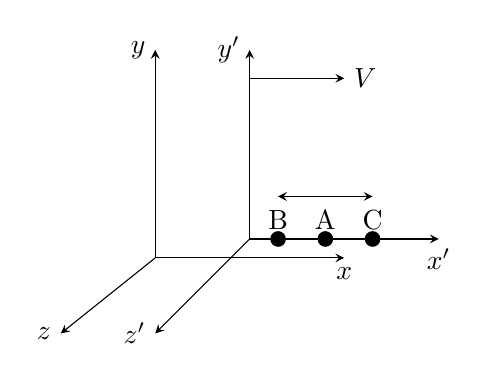
\begin{tikzpicture}[>=stealth,scale=1.2]

% Assi principali (sistema non primato)
\draw[->] (0,-0.2,0) -- (2,-0.2,0) node[below] {$x$};
\draw[->] (0,-0.2,0) -- (0,2,0) node[left] {$y$};
\draw[->] (0,-0.2,0) -- (-1,-1,0) node[left] {$z$};

% Assi primati
\draw[->] (1,0,0) -- (3,0,0) node[below] {$x'$};
\draw[->] (1,0,0) -- (1,2,0) node[left] {$y'$};
\draw[->] (1,0,0) -- (0,-1,0) node[left] {$z'$};

% Velocità V
\draw[->] (1,1.7,0) -- (2,1.7,0) node[right] {$V$};

% Punti
\node[circle,fill,inner sep=2pt] (B) at (1.3,0) {};
\node[circle,fill,inner sep=2pt] (A) at (1.8,0) {};
\node[circle,fill,inner sep=2pt] (C) at (2.3,0) {};

\node[above] at (B) {B};
\node[above] at (A) {A};
\node[above] at (C) {C};

% Frecce attorno ad A
\draw[<->] (1.3,0.45) -- (2.3,0.45);

\end{tikzpicture}
\caption{Sistemi di riferimento in moto relativo}
\label{fig:2_SistRef}
\end{figure}

L'ipotesi fondamentale della meccanica classica è il \textbf{tempo assoluto}, ovvero che il tempo scorra nello stesso modo per tutti gli osservatori inerziali ($t = t'$). In queste condizioni, le \textbf{Trasformazioni Galileiane di Posizione} si scrivono come:

\[
\begin{cases}
x = x' + vt \\
y = y' \\
z = z' \\
t = t'
\end{cases}
\]

Derivando queste relazioni rispetto al tempo, si ottengono le \textbf{Trasformazioni Galileiane di Velocità} o regola di composizione classica delle velocità:

\[
\begin{cases}
v_{x} = v'_{x} + v \\
v_{y} = v'_{y} \\
v_{z} = v'_{z}
\end{cases}
\]

Da queste relazioni, si evince che se una radiazione elettromagnetica viaggia con velocità $c$ lungo l'asse $x'$ nel sistema $K'$ (quindi $v'_{x} = c$), un osservatore nel sistema $K$ misurerebbe una velocità $v_x$ pari a $c + v$ (se $K'$ si allontana da $K$). Questa previsione, basata sul \textbf{Principio di Relatività Galileiana} e sull'ipotesi di \textbf{tempo assoluto}, è in \textbf{netto contrasto} con il risultato nullo dell'esperimento di Michelson-Morley e con la costanza della velocità della luce \cite{kittel1965meccanica}.

Questo profondo conflitto teorico-sperimentale evidenziò che l'ipotesi classica di $t=t'$ non è valida quando si considerano fenomeni ad alta velocità \cite{kittel1965meccanica}.

\section{Relatività ristretta}\label{relativita-ristretta}

Assumendo che il principio di relatività sia valido, all'inizio del '900 Einstein dimostrò che il concetto di tempo non è assoluto ma \textbf{relativo}. Egli si basò su due postulati fondamentali:

\begin{enumerate}
    \item Le leggi della fisica sono le stesse in tutti i sistemi di riferimento inerziali (Principio di Relatività).
    \item La velocità della luce nel vuoto ($c$) è la stessa in tutti i sistemi di riferimento inerziali, indipendentemente dal moto della sorgente o dell'osservatore (Principio di Invarianza di $c$).
\end{enumerate}

Si considerano due sistemi inerziali $K$ e $K'$, di cui il primo fermo, mentre il secondo in moto lungo la direzione delle $x$ positive con velocità costante $v$. Il secondo postulato di Einstein implica la non assolutezza del tempo. Per dimostrarlo, si considera l'esperimento mentale dei tre punti. Siano $A$, $B$ e $C$ tre punti sull'asse delle $x'$, con $A$ e $C$ equidistanti da $B$, sorgente luminosa. I tre punti sono solidali con il sistema di riferimento $K'$.

\begin{itemize}
    \item Per un osservatore solidale con $K'$: Egli vede i tre punti fermi. Poiché la luce procede con velocità $c$ in entrambe le direzioni e le distanze $BA$ e $BC$ sono uguali, la luce giunge \textbf{contemporaneamente} sui punti $A$ e $C$.
    \item Per un osservatore solidale con $K$: I tre punti si muovono con velocità $v$ nel verso positivo delle $x$. In particolare, $A$ si muove verso la luce emessa da $B$, mentre $C$ si allontana da essa. Poiché la velocità della luce deve essere $c$ anche in $K$, essa, dovendo percorrere cammini diversi, raggiunge prima il punto $A$ e, successivamente, il punto $C$.
\end{itemize}

Da questo esempio discende che, cambiando sistema di riferimento, gli eventi che in un sistema di riferimento $K'$ sono contemporanei, non lo sono nel sistema di riferimento $K$. Si conclude che la \textbf{simultaneità} è un concetto relativistico legato al sistema di riferimento considerato.

Per rispettare il principio di invarianza della velocità della luce, le trasformazioni tra i sistemi $K$ e $K'$ devono essere diverse da quelle galileiane. A tale scopo si supponga che un'onda luminosa sferica si propaghi partendo dall'origine dei due sistemi all'istante $t=t'=0\ \text{s}$ e si propaghi con velocità $c$. L'equazione che descrive il fronte d'onda deve essere la stessa nei due sistemi:

\[
\begin{cases}
x^{2} + y^{2} + z^{2} = r^{2} \\
{x'}^{2} + {y'}^{2} + {z'}^{2} = {r'}^{2}
\end{cases} 
\]

dove, i raggi sono dati da:

\[
r = ct, \quad \text{e} \quad r' = ct'
\]

Dato che gli assi $y$ e $z$ sono perpendicolari al moto, si ha $y=y'$ e $z=z'$. Per cui, è possibile scrivere:


\[
\begin{cases}
x^{2} + y^{2} + z^{2} = c^{2}t^{2} \\
{x'}^{2} + {y'}^{2} + {z'}^{2} = c^{2}{t'}^{2}
\end{cases} 
\]

Siccome gli eventi non sono simultanei nei due sistemi di riferimento, \(t' \neq t\).

Einstein postulò un legame di tipo lineare tra le coordinate, un'ipotesi necessaria per la ricerca della trasformazione, nella forma:

\[
\begin{cases}
x' = ax + bt \\
t' = gx + et
\end{cases}
\]

Si sostituisce queste relazioni nell'equazione che descrive l'espansione dell'onda in \(K'\):

\[
\left(ax + bt\right)^{2} + y^{2} + z^{2} = c^{2}\left(gx + et\right)^{2}
\]

Sviluppando i quadrati:

\[
a^{2}x^{2} + 2abxt + b^{2}t^{2} + y^{2} + z^{2} = c^{2}g^{2}x^{2} + 2c^{2}gext + c^{2}e^{2}t^{2}
\]

Raccogliendo, si ha:

\[
\left( a^{2} - c^{2}g^{2} \right)x^{2} + \left( 2ab - 2c^{2}ge \right)xt + y^{2} + z^{2} = \left( c^{2}e^{2} - b^{2} \right)t^{2}
\]

Questa equazione descrive l'onda nel sistema di riferimento \(K\), quindi, deve essere paragonata all'equazione:

\[
x^{2} + y^{2} + z^{2} = c^{2}t^{2}
\]

Questa equazione deve essere proporzionale a $x^{2} + y^{2} + z^{2} - c^{2}t^{2} = 0$. Uguagliando i coefficienti, si ottiene il sistema di equazioni:

\[
\begin{cases}
a^{2} - c^{2}g^{2} = 1 \quad \text{(coeff. di } x^2) \\
2ab - 2c^{2}ge = 0 \quad \text{(coeff. di } xt) \\
c^{2}e^{2} - b^{2} = c^{2} \quad \text{(coeff. di } t^2)
\end{cases}
\]

Il sistema ottenuto presenta tre equazioni, nelle incognite $a$, $b$, $e$ e $g$. È, dunque, necessario aggiungere una quarta equazione che leghi i coefficienti alla velocità relativa $v$. A tale scopo, si considera un punto fermo nel sistema $K'$, per il quale $dx' = 0$. Dalla trasformazione di $x'$, differenziando, si ha:

\[
dx' = a\ dx + b\ dt = 0 \Leftrightarrow \dfrac{dx}{dt} = - \dfrac{b}{a}
\]

La quantità $dx/dt$ è la velocità di un punto fermo in $K'$ misurata in $K$. Poiché il sistema $K'$ si muove rispetto a $K$ con velocità $v$, si deve avere:

\[
\dfrac{dx}{dt} = v
\]

Pertanto, è valida la relazione:

\[
v = - \dfrac{b}{a} \Leftrightarrow b = -av
\]

Si ottiene il sistema risolvibile:

\[
\begin{cases}
a^{2} - c^{2}g^{2} = 1 \quad \text{(Eq. 1)} \\
ab - c^{2}ge = 0 \quad \text{(Eq. 2)} \\
c^{2}e^{2} - b^{2} = c^{2} \quad \text{(Eq. 3)} \\
b = - av \quad \text{(Eq. 4)}
\end{cases}
\]

Si considera la terza equazione:

\[c^{2}e^{2} - b^{2} = c^{2}\]

Si sostituisce l'ultima:

\[c^{2}e^{2} - v^{2}e^{2} = c^{2}\]

Da cui è possibile ricavare \(e\):

\[e^{2} = \dfrac{c^{2}}{c^{2} - v^{2}} = \dfrac{1}{1 - \left( \dfrac{v}{c} \right)^{2}}\]

\[e = \dfrac{1}{\sqrt{1 - \left( \dfrac{v}{c} \right)^{2}}}\]

Noto \(e\) è possibile risalire a \(b\) dalla quarta equazione:

\[b = - ve = - \dfrac{v}{\sqrt{1 - \left( \dfrac{v}{c} \right)^{2}}}\]

Dalla seconda equazione è possibile ricavare \(g\) in funzione di \(a\):

\[c^{2}ge = ab \Leftrightarrow g = \dfrac{1}{c^{2}}a\dfrac{b}{e}\]

Per la quarta equazione, si ha:

\[g = - \dfrac{v}{c^{2}}a\]

Si sostituisce questo risultato nella prima equazione:

\[a^{2} - c^{2}g^{2} = 1 \Leftrightarrow a^{2} - c^{2}\dfrac{v^{2}}{c^{4}}a^{2} = 1 \Leftrightarrow \left( 1 - \dfrac{v^{2}}{c^{2}} \right)a^{2} = 1 \Leftrightarrow a = \dfrac{1}{\sqrt{1 - \left( \dfrac{v}{c} \right)^{2}}}\]

Noto \(a\), è possibile risalire a \(g\):

\[g = - \dfrac{v}{c^{2}}a = - \dfrac{v}{c^{2}}\dfrac{1}{\sqrt{1 - \left( \dfrac{v}{c} \right)^{2}}}\]

I coefficienti determinati sono, dunque:

\[
\begin{cases}
a = \dfrac{1}{\sqrt{1 - \left( \dfrac{v}{c} \right)^{2}}} \\
b = - \dfrac{v}{\sqrt{1 - \left( \dfrac{v}{c} \right)^{2}}} \\
g = - \dfrac{v}{c^{2}}\dfrac{1}{\sqrt{1 - \left( \dfrac{v}{c} \right)^{2}}} \\
e = \dfrac{1}{\sqrt{1 - \left( \dfrac{v}{c} \right)^{2}}}
\end{cases}
\]

Dato che il rapporto della velocità di movimento del sistema di riferimento sulla velocità della luce compare frequentemente, si pone:

\[
\dfrac{v}{c} = \beta
\]

La quantità:

\[
\gamma = \dfrac{1}{\sqrt{1 - \left( \dfrac{v}{c} \right)^{2}}} = \dfrac{1}{\sqrt{1 - \beta^{2}}}
\]

È detto \textbf{fattore di Lorentz}. Con queste definizioni, i coefficienti delle equazioni di composizione possono essere scritti come:

\[
\begin{cases}
a = \gamma \\
b = - v\gamma \\
 g = - \dfrac{v}{c^{2}}\gamma \\
e = \gamma
\end{cases} \Leftrightarrow \begin{cases}
a = \gamma \\
b = - \beta\gamma c \\
 g = - \dfrac{\beta}{c}\gamma \\
e = \gamma
\end{cases} 
\]

Le leggi di trasformazioni tra il sistema \(K\) e \(K'\) sono dette \textbf{trasformazioni di Lorentz} e sono \cite{landau1975campi,feynman1964vol1}:

\[
\begin{cases}
x' = ax + bt \\
y' = y \\
z' = z \\
t' = gx + et
\end{cases} \Leftrightarrow \begin{cases}
x' = \gamma (x - vt) \\
y' = y \\
z' = z \\
t' = \gamma \left( t - \dfrac{vx}{c^{2}} \right)
\end{cases}
\]

\subsection{Composizione delle velocità}\label{composizione-delle-velocituxe0}

Si determinano, ora, le leggi di trasformazione per la velocità; a tale scopo si differenziano le trasformazioni di Lorentz:

\[
\begin{cases}
dx' = \gamma (dx - v\,dt) \\
dy' = dy \\
dz' = dz \\
dt' = \gamma \left( dt - \dfrac{v}{c^{2}}\,dx \right)
\end{cases}
\]

Dividendo una delle variazioni spaziali per $dt'$ si ottengono le velocità lungo gli assi nel sistema $K'$.

La velocità $v_{x'}$ è data dal rapporto $dx'/dt'$. Sostituendo le espressioni differenziali:
\[
v_{x'} = \dfrac{dx'}{dt'} = \dfrac{\gamma(dx - v\,dt)}{\gamma\left( dt - \dfrac{v}{c^{2}}\,dx \right)} = \dfrac{dx - v\,dt}{dt - \dfrac{v}{c^{2}}\,dx}
\]

Al secondo membro si divide numeratore e denominatore per $dt$ per far comparire le velocità $v_x = dx/dt$:

\[
v_{x'} = \dfrac{\dfrac{dx}{dt} - v}{1 - \dfrac{v}{c^{2}}\dfrac{dx}{dt}}
\]

Posto $v_{x} = dx/dt$ come la componente di velocità lungo l'asse \(x\) con cui si muove un fenomeno nel sistema \(K\), si ottiene la formula di composizione relativistica:

\[
v_{x'} = \dfrac{v_{x} - v}{1 - \dfrac{v_{x}v}{c^{2}}}
\]

Lungo \(y'\), la velocità è data da:

\[
v_{y'} = \dfrac{dy'}{dt'} = \dfrac{dy}{\gamma\left( dt - \dfrac{v}{c^{2}}\,dx \right)}
\]

Moltiplicando e dividendo per \(dt\) al secondo membro, si ha:

\[
v_{y'} = \dfrac{\dfrac{dy}{dt}}{\gamma\left( 1 - \dfrac{v}{c^{2}}\dfrac{dx}{dt} \right)}
\]

Dove compare la componente di velocità lungo l'asse \(x\) con cui si muove un fenomeno nel sistema \(K\):

\[
\dfrac{dy}{dt} = v_{y} \Rightarrow v_{y'} = \dfrac{v_{y}}{\gamma\left( 1 - \dfrac{v_{x}v}{c^{2}} \right)}
\]

Analogamante, per la componente lungo \(z'\) si ha:

\[
v_{z'} = \dfrac{dz'}{dt'} = \dfrac{dz}{\gamma\left( dt - \dfrac{v}{c^{2}}\,dx \right)} = \dfrac{v_{z}}{\gamma\left( 1 - \dfrac{v_{x}v}{c^{2}} \right)}
\]

Si considera il caso in cui la velocità $v_{x} = c$ (un raggio di luce nel sistema $K$). Nel sistema $K'$, la velocità $v_{x'}$ diventa:

\[
v_{x'} = \left. \ \dfrac{v_{x} - v}{1 - \dfrac{v_{x}v}{c^{2}}} \right|_{v_{x} = c} = \dfrac{c - v}{1 - \dfrac{cv}{c^{2}}} = \dfrac{c - v}{1 - \dfrac{v}{c}} = \dfrac{c - v}{\dfrac{c - v}{c}} = c
\]

Le trasformazioni di Lorentz per la composizione delle velocità verificano, quindi, il \textbf{Principio di Invarianza della Velocità della Luce}, risolvendo la contraddizione presente nelle leggi di composizione galileiane.

\subsection{Fattore di Lorentz}\label{fattore-di-lorentz}

Il \textbf{fattore di Lorentz} ($\gamma$) è definito come:

\[
\gamma = \dfrac{1}{\sqrt{1 - \left( \dfrac{v}{c} \right)^{2}}}
\]

dove $v$ è la velocità relativa tra i sistemi di riferimento e $c$ è la velocità della luce.

Le velocità considerate nella maggior parte delle applicazioni pratiche sono molto minori della velocità della luce:

\[
\dfrac{v}{c} \ll 1
\]

In questo caso, il fattore $\left(v/c\right)^{2}$ è trascurabile, e il fattore di Lorentz tende all'unità:

\[
\gamma \simeq 1 \quad \text{per } v \ll c
\]

In questo limite, la relatività ristretta ricade nella \textbf{meccanica classica} (o meccanica newtoniana). La meccanica classica, in ultima analisi, è un caso particolare della meccanica relativistica di Einstein, valido quando gli effetti relativistici sono minimi.

Al crescere della velocità $v$, il fattore di Lorentz, sempre positivo, tende a crescere. Nel caso limite in cui la velocità si avvicina alla velocità della luce ($v \rightarrow c$), il denominatore tende a zero:

\[
\lim_{v \to c} \gamma = \lim_{v \to c} \dfrac{1}{\sqrt{1 - \left( \dfrac{v}{c} \right)^{2}}} \rightarrow \infty
\]

\begin{figure}[h!]
\centering
\begin{figure}[h!]
\centering
\begin{tikzpicture}

\begin{axis}[
    axis lines=middle,
    xlabel={$V$},
    ylabel={$\gamma$},
    xmin=0, xmax=1.2,
    ymin=1, ymax=6,
    xtick={0.2,0.4,0.6,0.8, 1},
    xticklabels={$0.2c$, $0.4c$, $0.6c$, $0.8c$, $c$},
    ytick={1},
    domain=0:0.99,
    samples=200,
    smooth,
    width=11cm,
    height=7cm,
    axis line style={->},
    tick style={black},
]

% Curva gamma
\addplot[black, thick] {1/sqrt(1-x^2)};

% Linea tratteggiata vicino a c
\draw[dashed] (axis cs:0.99,0) -- (axis cs:0.99,10);

\end{axis}

\end{tikzpicture}
\caption{Andamentodel fattorediLorentz al variare della velocità}
\label{fig:2_GammaFactor}
\end{figure}
\caption{Andamento del fattore di Lorentz al variare della velocità}
\label{fig:2_GammaFactor}
\end{figure}


La velocità della luce ($c$) rappresenta un \textbf{limite irraggiungibile} per qualsiasi corpo massivo secondo la meccanica relativistica.

\subsection{Dilatazione dei tempi}\label{dilatazione-dei-tempi}

Si considerano due sistemi di riferimento inerziali \(K\) e \(K'\), in moto relativo tra loro con velocità \(v\) lungo la direzione delle \(x\) positive. Si suppone che \(K\) sia fermo.

Per ricavare $dt$ in funzione di $dt'$ e $dx'$, si parte dalle Trasformazioni di Lorentz:

\[
\begin{cases}
dx' = \gamma(dx - \beta c)dt \\
dy' = dy \\
dz' = dz \\
dt' = \gamma\left( - \dfrac{\beta}{c}dx + dt \right)
\end{cases}
\]

Si considerano solamente la prima e la quarta equazione. Tramite queste si ricavano le coordinate del sistema di riferimento fisso \(K\) in funzione di quelle relative a \(K'\)

\[
\begin{cases}
dx' = \gamma(dx - \beta c)dt \\
dt' = \gamma\left( - \dfrac{\beta}{c}dx + dt \right)
\end{cases}  \Leftrightarrow \begin{cases}
\dfrac{1}{\gamma}dx' = dx - \beta c\ dt \\
\dfrac{1}{\gamma}dt' = - \dfrac{\beta}{c}\ dx + dt
\end{cases} \Leftrightarrow \begin{cases}
dx = \dfrac{1}{\gamma}dx' + \beta c\ dt \\
dt = \dfrac{1}{\gamma}dt' + \dfrac{\beta}{c}\ dx
\end{cases}
\]

Si sostituisce la prima equazione nella seconda:

\[
dt = \dfrac{1}{\gamma}dt' + \dfrac{\beta}{c}\ dx \Leftrightarrow dt = \dfrac{1}{\gamma}dt' + \dfrac{\beta}{c}\ \left( \dfrac{1}{\gamma}dx' + \beta c\ dt \right)
\]

Risolvendo, si ha:

\[
dt = \dfrac{1}{\gamma}dt' + \dfrac{\beta}{\gamma c}\ dx' + \beta^{2}dt
\]

Si portano i termini contenenti \(dt\) al primo membro:

\[
\left( 1 - \beta^{2} \right)dt = \dfrac{1}{\gamma}dt' + \dfrac{\beta}{\gamma c}\ dx'
\]

Isolando \(dt\), si ha:

\[
dt = \dfrac{1}{\gamma\left( 1 - \beta^{2} \right)}\left( dt' + \dfrac{\beta}{c}\ dx' \right)
\]

Per definizione, il fattore di Lorentz può essere scritto come:

\[
\gamma = \dfrac{1}{\sqrt{1 - \beta^{2}}}
\]

Sostituendo questo risultato nell'espressione per \(dt\) si ottiene:

\[
dt = \dfrac{\sqrt{1 - \beta^{2}}}{\left( 1 - \beta^{2} \right)}\left( dt' + \dfrac{\beta}{c}\ dx' \right) = \dfrac{1}{\sqrt{1 - \beta^{2}}}\left( dt' + \dfrac{\beta}{c}\ dx' \right) = \gamma\left( dt' + \dfrac{\beta}{c}\ dx' \right)
\]

Noto \(dt\), è possibile ricavare \(dx\) dalla prima equazione:

\[
dx = \dfrac{1}{\gamma}dx' + \beta c\ dt = \dfrac{1}{\gamma}dx' + \beta c\gamma\left( dt' + \dfrac{\beta}{c}\ dx' \right) = \dfrac{1}{\gamma}dx' + \beta c\gamma\ dt' + \beta^{2}\gamma\ dx'
\]

Si raccoglie \(\gamma\) al secondo membro:

\[
dx = \gamma\left\lbrack \left( \dfrac{1}{\gamma^{2}} + \beta^{2} \right)dx' + \beta c\ dt' \right\rbrack
\]

Dove, per definizione del fattore di Lorentz:

\[
\dfrac{1}{\gamma^{2}} + \beta^{2} = 1 - \beta^{2} + \beta^{2} = 1
\]

Con questo risultato, si ottiene l'espressione per \(dx\):

\[
dx = \gamma\left( dx' + \beta c\ dt' \right)
\]

Le due equazioni, per \(dx\) e \(dt\), sono, in definitiva:

\[
\begin{cases}
dx = \gamma\left( dx' + \beta c\ dt' \right) \\
dt = \gamma\left( dt' + \dfrac{\beta}{c}\ dx' \right)
\end{cases}
\]

Si considera un orologio o un fenomeno solidale col sistema di riferimento \(K'\), ovvero fermo rispetto a esso. Ne discende che \(dx' = 0\), in quanto la variazione lungo l'asse \(x\) è nulla, essendo, appunto, il punto fermo. Nel sistema di riferimento \(K\), la variazione temporale è data da:

\[
dt = \left. \gamma\left( dt' + \dfrac{\beta}{c}\ dx' \right) \right|_{dx' = 0} = \gamma\ dt'
\]

Si definisce tempo proprio \(\tau\) il tempo che una particela vede scorrere nel sistema di riferimento in cui è in quiete. Con questa definizione, la relazione può essere scritta come:

\[
dt = \gamma\ d\tau
\]

L'intervallo di tempo $dt$ misurato in $K$ (dove l'orologio è in moto) è maggiore dell'intervallo di tempo proprio $d\tau$ (dove l'orologio è fermo). Ciò significa che, per l'osservatore in $K$, \textbf{gli orologi in movimento scorrono più lentamente} del suo orologio. Questo è l'effetto noto come dilatazione dei tempi.

Per apprezzare tale effetto, noto come dilatazione dei tempi, il fattore di Lorentz \(\gamma\) deve essere significativamente maggiore di \(1\). Tale condizione si verifica quando la velocità con cui si muove \(K'\) rispetto a \(K\) deve essere prossima alla velocità della luce.

Per apprezzare tale effetto, il fattore di Lorentz \(\gamma\) deve essere significativamente maggiore di \(1\).

\begin{itemize}
 \item \textbf{Limite Classico} ($v \ll c$): In questo limite, il fattore di Lorentz è circa unitario ($\gamma \simeq 1$), dunque la dilatazione dei tempi non è apprezzabile:
    
 \[
 dt \simeq d\tau
 \]
 \item \textbf{Limite Relativistico} ($v \to c$): Nel caso limite in cui \(K'\) si muove alla velocità della luce, il fattore di Lorentz tende all'infinito ($\gamma \to \infty$):
 \[
 dt = \left. \ \gamma\ d\tau \right|_{v \to c} \rightarrow \infty
 \]
    Ciò implica che, per un osservatore esterno, il tempo di un oggetto che viaggia alla velocità della luce (se fosse possibile) si fermerebbe.
\end{itemize}

A differenza degli intervalli di tempo misurati nei vari sistemi di riferimento, il tempo proprio \(\tau\) è univocamente determinato noto \(\gamma\), ovvero la velocità relativa di \(K'\) rispetto al sistema di riferimento \(K\), in cui si effettua la misura.

\subsection{Contrazione delle lunghezze}\label{contrazione-delle-lunghezze}

Si considerino due sistemi di riferimento inerziali $K$ e $K'$, in moto relativo con velocità $v$ (con $\beta = v/c$) lungo la direzione positiva dell'asse $x$. Si assuma che il sistema $K$ sia fermo e si osservano due punti nel sistema $K'$ nello stesso istante; pertanto la variazione temporale è nulla: $dt' = 0$.

Nel sistema in moto $K'$ si misura una distanza $dx'$, mentre un osservatore nel sistema fisso $K$ misura una distanza $dx$, legata a $dx'$ dalle trasformazioni di Lorentz:

\[
\begin{cases}
dx = \gamma\left( dx' + \beta c\ dt' \right) \\
 dt = \gamma\left( dt' + \dfrac{\beta}{c}\ dx' \right)
\end{cases} 
\]

dove $\gamma = 1/\sqrt{1-\beta^2}$.

Per misurare la lunghezza di un oggetto in movimento, l'osservatore nel sistema $K$ deve determinare le posizioni delle sue estremità simultaneamente nel proprio sistema, cioè $dt=0$. Impostando quindi la seconda equazione a zero si ottiene:

\[
dt = \gamma\left( dt' + \dfrac{\beta}{c}\ dx' \right) \Leftrightarrow\ \gamma\left( dt' + \dfrac{\beta}{c}\ dx' \right) = 0
\]

Da cui si ricava:

\[
dt' = - \dfrac{\beta}{c}\ dx'
\]

Sostituendo questo risultato nella prima equazione:

\[
dx = \gamma\left( dx' + \beta c\, dt' \right)
     = \gamma\left( dx' + \beta c \left( - \dfrac{\beta}{c}\, dx' \right) \right)
     = \gamma\left( dx' - \beta^2 dx' \right).
\]

Raccogliendo $dx'$:

\[
dx = \gamma\, dx' (1 - \beta^2).
\]

Poiché $1 - \beta^2 = \gamma^{-2}$, si ottiene:

\[
dx = \gamma dx' \left(\dfrac{1}{\gamma^2}\right) 
\]

Semplificando $\gamma$ si ottiene la relazione che lega la lunghezza nel sistema $K$, ovvero $dx$, con quella nel sistema $K'$, $dx'$:

\[
dx = \dfrac{1}{\gamma} dx'
\]

Poiché \(\gamma > 1,v > 0\), la lunghezza misurata nel sistema $K$, in cui l'oggetto è in moto, risulta dunque minore rispetto alla misura $dx'$ ottenuta nel sistema $K'$, in cui l'oggetto è in quiete. La distanza tra due punti è massima nel sistema in cui essi sono fermi; inoltre, a differenza delle misure ottenute negli altri sistemi, essa è univocamente determinata noto $\gamma$, cioè la velocità relativa tra i sistemi.

Infine, noto $\gamma$ e $dx'$, è sempre possibile determinare la corrispondente misura $dx$ in qualsiasi sistema di riferimento inerziale.

\subsection{Energia e quantità di moto relativistiche}\label{energia-e-quantituxe0-di-moto-relativistiche}

Si ricavano le relazioni di energia e quantità di moto nella teoria della Relatività Ristretta partendo dal \textbf{Principio di Azione Stazionaria} (o di Hamilton). L'azione $S$ di una particella libera è definita come l'integrale della Lagrangiana $L$ rispetto al tempo coordinato $t$:

\[
S = \int_{t_1}^{t_2}{L dt}
\]

L'azione $S$ deve essere uno \textbf{scalare di Lorentz}, ovvero deve avere lo stesso valore in tutti i sistemi di riferimento inerziali. Affinché $S$ sia invariante, la Lagrangiana $L$ non può essere una semplice estensione della Lagrangiana classica.

Si osserva che l'elemento di linea $ds$ e il \textbf{tempo proprio} $d\tau$ sono invarianti di Lorentz: 

\[
ds^2 = c^2 dt^2 - d\mathbf{x} \cdot d\mathbf{x} = c^2 d\tau^2
\]

Il tempo proprio $d\tau$ è legato al tempo misurato in un sistema di riferimento inerziale ($dt$) tramite il fattore di Lorentz $\gamma$:

\[
d\tau = \frac{1}{\gamma} dt = \sqrt{1 - \frac{v^{2}}{c^{2}}}dt
\]

Per garantire l'invarianza dell'azione, l'integrando deve essere una quantità proporzionale al tempo proprio, l'unico intervallo di tempo intrinsecamente legato alla particella. Si definisce l'azione come: 

\[
S = \int_{\tau_1}^{\tau_2}{\alpha d\tau}
\]

dove $\alpha$ è una costante scalare da determinare.

Sostituendo l'espressione per $d\tau$, l'azione può essere riscritta in funzione del tempo coordinato $t$:

\[
S = \int_{t_1}^{t_2}{\alpha \sqrt{1 - \frac{v^{2}}{c^{2}}}dt}
\]

Da cui si ricava la \textbf{Lagrangiana Relativistica} $L^{r}$: 

\[
L^{r} = \alpha \sqrt{1 - \frac{v^{2}}{c^{2}}}
\]

La meccanica relativistica deve inglobare la meccanica classica nel caso limite in cui $v \ll c$. In questa condizione, la Lagrangiana relativistica approssimata $L_{appr}^{r}$ deve coincidere con la Lagrangiana classica $L_{class}$, a meno di una costante additiva. 
Per $v \ll c$, usiamo l'approssimazione binomiale: 

\[
\sqrt{1 - \dfrac{v^{2}}{c^{2}}} \simeq 1 - \dfrac{1}{2}\dfrac{v^{2}}{c^{2}},\ \ v \ll c
\] 

Con questo risultato l'azione, nel limite classico, può essere scritta come:

\[
S = \int{\alpha\sqrt{1 - \dfrac{v^{2}}{c^{2}}}dt} \simeq \int{\alpha\left( 1 - \dfrac{1}{2}\dfrac{v^{2}}{c^{2}} \right)dt}
\]

L'integrando coincide con la lagrangiana relativistica $L_{appr}^r$, nel limite delle meccanica classica, in cui le velocità in gioco sono molto minori della velocità della luce. Questa quantità deve coincidere con la lagrangiana classica ($L_{class}$), a meno di una costante additiva, in quanto le equazioni di Eulero-Lagrange dipendono solamente dalla derivata della lagrangiana.

Per una particella libera, la Lagrangiana classica è:

\[
L_{class} = \frac{1}{2}m_{0}v^{2}
\]

dove $m_{0}$ è la \textbf{massa a riposo} (o massa invariante). Nell'approssimazione classica, l'azione è data da:

\[
S_{class} = \int{L_{class}dt} = \int{\dfrac{1}{2}m_{0}v^{2}dt}
\]

Confrontando le Lagrangiane nel limite classico, si pone l'uguaglianza dei termini dipendenti da $v^2$: 

\[ 
L_{appr}^{r} = \alpha - \dfrac{1}{2}\alpha\dfrac{v^{2}}{c^{2}} 
\]

La costante \(\alpha\) non influenza l'equazione di Eulero-Lagrange, dunque può essere trascurata. Deve valere: 

\[ 
- \dfrac{1}{2}\alpha\dfrac{v^{2}}{c^{2}} = \dfrac{1}{2}m_{0}v^{2} 
\] 

Da cui si ricava \(\alpha\) come:

\[\alpha = - m_{0}c^{2}\]

Sostituendo $\alpha$, la Lagrangiana approssimata diventa: 

\[ 
L_{appr}^r = - m_{0}c^{2}\left( 1 - \dfrac{1}{2}\dfrac{v^{2}}{c^{2}} \right) = \underbrace{- m_{0}c^{2}}_{\text{costante}} + \underbrace{\dfrac{1}{2}m_{0}v^{2}}_{L_{class}} 
\] 

La costante $- m_{0}c^{2}$ non influenza le equazioni del moto di Eulero-Lagrange e, dunque, la Lagrangiana relativistica per una particella libera è: 

\[ 
L^{r} = - m_{0}c^{2}\sqrt{1 - \dfrac{v^{2}}{c^{2}}} = - m_{0}c^{2}\sqrt{1 - \dfrac{\mathbf{v} \cdot \mathbf{v}}{c^{2}}} 
\]

Con questo risultato si ha la certezza che, nel limite \(v \ll c\), la lagrangiana relativistica e quella classica coincidano, a meno di una costante \(- m_{0}c^{2}\).

Dall'equivalenza tra meccanica newtoniana e meccanica lagrangiana è possibile ricavare la definizione di momento lineare generalizzato alla meccanica relativistica:

\[
\mathbf{p} = \dfrac{\partial L}{\partial\mathbf{v}} = \dfrac{\partial}{\partial\mathbf{v}}\left( - m_{0}c^{2}\sqrt{1 - \dfrac{\mathbf{v} \cdot \mathbf{v}}{c^{2}}} \right) = \dfrac{m_{0}\mathbf{v}}{\sqrt{1 - \dfrac{v^{2}}{c^{2}}}}
\]

Semplificando i termini, si ottiene la \textbf{quantità di moto relativistica}: 

\[ 
\mathbf{p} = \dfrac{m_{0}\mathbf{v}}{\sqrt{1 - \dfrac{v^{2}}{c^{2}}}} = \gamma m_{0}\mathbf{v} 
\] 

dove $\gamma = \frac{1}{\sqrt{1 - v^2/c^2}}$ è il fattore di Lorentz. 

Da questa relazione è possibile osservare che la massa relativistica è legata alla massa inerziale dalla relazione:

\[
m = \dfrac{m_{0}}{\sqrt{1 - \dfrac{v^{2}}{c^{2}}}} = \gamma m_{0}
\]

dove \(m_{0}\) è detta massa a riposo e rappresenta la quantità di materia che possiede un corpo da fermo. La massa \(m\) di una particella dipende, invece, dalla velocità con cui si muove. Nel limite classico, \(v \ll c\), il fattore di Lorentz è prossimo all'unità, per cui, la massa relativistica \(m\) coincide con la massa a riposo:

\[
m \simeq m_{0},\ \ v \ll c
\]

Se la velocità \(v\) tende a raggiungere la velocità della luce, il fattore di Lorentz tende a diventare infinito; di conseguenza, anche la massa relativistica tende a divergere:

\[
m \rightarrow \infty,\quad v \rightarrow c
\]

\begin{figure}[ht]
\centering
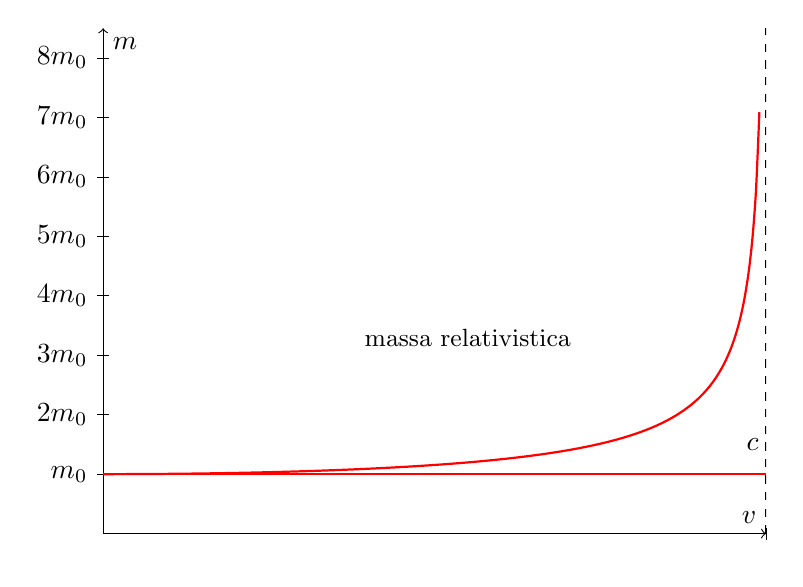
\begin{tikzpicture}

\begin{axis}[
    axis lines=middle,
    xlabel={$v$},
    ylabel={$m$},
    xmin=0, xmax=1,
    ymin=0, ymax=8.5,
    xtick={1},
    xticklabels={},
    ytick={1,2,3,4,5,6,7,8},
    yticklabels={$m_0$, $2m_0$, $3m_0$, $4m_0$, $5m_0$, $6m_0$, $7m_0$, $8m_0$},
    width=10cm,
    height=8cm,
    domain=0:0.99,
    samples=200,
    smooth,
    axis line style={->},
    tick style={black},
]

% Curva massa relativistica m = gamma m0
\addplot[red, thick] {1/sqrt(1 - x^2)};

% Linea orizzontale della massa a riposo
\addplot[red, thick] coordinates {(0,1) (1,1)};

% Linea verticale in v = c
\draw[dashed] (axis cs:1,0) -- (axis cs:1,8.5);

% Etichetta "massa relativistica"
\node at (axis cs:0.55,3.3) {\small massa relativistica};

% Etichetta "c" posizionata più in alto
\node at (axis cs:0.98,1.5) {$c$};

\end{axis}

\end{tikzpicture}


\caption{Andamento della massa relativistica in funzione della velocità}
\label{fig:2_MassRelav}
\end{figure}

La divergenza della massa relativistica al crescere della velocità spiega perché non sia possibile superare la velocità della luce \(c\). Infatti, l'energia fornita a una particella in parte ne aumenta la velocità e in parte ne accresce la massa relativistica. Di conseguenza, per superare la velocità della luce \(c\) è necessario fornire un'energia infinita, il che è fisicamente impossibile.

La quantità di moto, a differenza del limite classico, è legata alla massa relativistica, che a sua volta dipende dalla velocità. Di conseguenza, la quantità di moto non dipende più in modo lineare dalla velocità:

\[
\mathbf{p} = m\mathbf{v}
\]

Essa presenta, invece, una relazione più complessa, poiché anche la massa dipende dalla velocità:

\[
\mathbf{p} = \dfrac{m_{0}\mathbf{v}}{\sqrt{1 - \dfrac{v^{2}}{c^{2}}}}
\]

La massa \(m\), nel piano \(p - v\), rappresenta la pendenza della curva quantità di moto in funzione della velocità. Nella teoria relativistica, non si ha una retta. L'andamento della quantità di moto relativistica è lineare nel limite classico, dunque per \(v \ll c\).

\begin{figure}[h!]
\centering
\input{Image/2_Relatività/2_qMotoRelativistica}
\caption{Andamento della quantità di moto relativistica}
\label{fig:2_qMotoRelativistica}
\end{figure}

L'energia totale $E$ per un sistema non dipendente esplicitamente dal tempo è data dall'Hamiltoniana $H$, che in meccanica lagrangiana è definita come:

\[ 
E = H = \dfrac{\partial L}{\partial\mathbf{v}} \cdot \mathbf{v} - L = \mathbf{p} \cdot \mathbf{v} - L^{r} 
\]

Sostituendo le espressioni ricavate per la quantità di moto $\mathbf{p}$ e la Lagrangiana $L^{r}$:

\[ 
E = \left( \dfrac{m_{0}\mathbf{v}}{\sqrt{1 - \dfrac{v^{2}}{c^{2}}}} \right) \cdot \mathbf{v} - \left( - m_{0}c^{2}\sqrt{1 - \dfrac{v^{2}}{c^{2}}} \right) 
\]

Svolgendo il prodotto scalare, si ottiene:

\[ 
E = \dfrac{m_{0}v^{2}}{\sqrt{1 - \dfrac{v^{2}}{c^{2}}}} + m_{0}c^{2}\sqrt{1 - \dfrac{v^{2}}{c^{2}}} 
\]

Si esegue il minimo comune multiplo al secondo membro e, successivamente, si svolgono i prodotti:

\[
E = \dfrac{m_{0}v^{2} + m_{0}c^{2}\left( 1 - \dfrac{v^{2}}{c^{2}} \right)}{\sqrt{1 - \dfrac{v^{2}}{c^{2}}}} = \dfrac{m_{0}v^{2} + m_{0}c^{2} - m_{0}v^{2}}{\sqrt{1 - \dfrac{v^{2}}{c^{2}}}}
\]

L'energia totale è, quindi, la celebre relazione: 
\[ 
E = \dfrac{m_{0}c^{2}}{\sqrt{1 - \dfrac{v^{2}}{c^{2}}}} = \gamma m_{0}c^{2} 
\]

Questa relazione rappresenta una delle equazioni più note di Einstein e della relatività ristretta \cite{landau1994meccanica,feynman1964vol1}. Il termine \(m_{0}c^{2}\) rappresenta un termine energetico, legato allo stato di quiete della particella. Infatti, nel limite classico, è possibile approssimare in serie di Taylor il denominatore:

\[
\dfrac{1}{\sqrt{1 - \dfrac{v^{2}}{c^{2}}}}\simeq 1 + \dfrac{1}{2}\dfrac{v^{2}}{c^{2}}
\]

Sostituendo tale risultato nell'equazione per l'energia $E$, si ottiene:

\[
E = \dfrac{m_{0}}{\sqrt{1 - \dfrac{v^{2}}{c^{2}}}}c^{2}\simeq m_{0}c^{2}\left(1 + \dfrac{1}{2}\dfrac{v^{2}}{c^{2}}\right)
\]

Svolgendo i prodotti, si ricava l'espressione per l'energia totale nel limite classico:

\[
E\simeq m_{0}c^{2} +\dfrac{1}{2}m_{0}v^{2} ,\ \ v \ll c
\]

L'energia totale della particella è la somma dell'\textbf{Energia a Riposo} ($E_0 = m_{0}c^{2}$) e dell'\textbf{Energia Cinetica Classica} per una particella libera. 

L'\textbf{Energia Cinetica Relativistica} $K$ è definita come la differenza tra l'energia totale e l'energia a riposo: 

\[ 
K = E - E_0 = \gamma m_{0}c^{2} - m_{0}c^{2} = m_{0}c^{2} (\gamma - 1) 
\]

Se la velocità $v$ approssima quella della luce, il fattore $\gamma \rightarrow \infty$, e di conseguenza anche l'energia totale $E \rightarrow \infty$. Questo risultato implica che è \textbf{impossibile} accelerare una particella con massa a riposo non nulla fino alla velocità della luce, poiché richiederebbe un apporto energetico infinito. 

Anche in meccanica relativistica valgono i teoremi di conservazione, tuttavia, i principi di conservazione della massa e dell'energia sono sostituiti dal principio di conservazione della massa-energia.

Elevando al quadrato l'equazione dell'energia totale e della quantità di moto ($p=|\mathbf{p}|$), si ottiene una relazione fondamentale che non dipende dalla velocità:

\[
\begin{cases} 
E^2 &= \dfrac{m_{0}^{2}c^{4}}{1 - \dfrac{v^{2}}{c^{2}}} \\ 
(p c)^2 &= \dfrac{m_{0}^{2}v^{2}c^{2}}{1 - \dfrac{v^{2}}{c^{2}}} 
\end{cases} 
\]

Sottraendo la seconda dalla prima: 

\[ 
E^2 - (pc)^2 = \dfrac{m_{0}^{2}c^{4} - m_{0}^{2}v^{2}c^{2}}{1 - \dfrac{v^{2}}{c^{2}}} = \dfrac{m_{0}^{2}c^{4} \left( 1 - \dfrac{v^{2}}{c^{2}} \right)}{1 - \dfrac{v^{2}}{c^{2}}} 
\] 

Da cui si ricava la \textbf{Relazione Energia-Quantità di Moto}: 

\[ 
E^2 = (pc)^2 + (m_{0}c^2)^2 
\] 

Questa relazione mostra come $m_{0}c^2$ sia una quantità invariante di Lorentz, proprio come la lunghezza del quadrivettore energia-quantità di moto $(E/c, \mathbf{p})$. 

\section{Quadrivettori}\label{quadrivettori}

Lo \textbf{spazio-tempo di Minkowski} o \textbf{cronotopo} è lo spazio quadridimensionale introdotto da Einstein nella relatività ristretta, composto da tre coordinate spaziali e una temporale. Ogni fenomeno fisico è descritto da eventi nello spazio-tempo, detti quadrivettori.

Il quadrivettore posizione $\mathbf{x}^{\mu}$ è:

\[ 
{x}^{\mu} = \begin{pmatrix} 
ct, x, y, z 
\end{pmatrix} 
\] 

è necessario introdurre come prima componente $ct$ (dove $x^0 = ct$) in modo da avere delle quantità dimensionalmente omogenee. 

Si definisce \textbf{intervallo spazio-temporale} $\Delta s^2$ la quantità (invariante di Lorentz):

\[ 
\Delta s^{2} = c^{2}\Delta t^{2} - \left( \Delta x^{2} + \Delta y^{2} + \Delta z^{2} \right) 
\] 

Il termine $\Delta x^{2} + \Delta y^{2} + \Delta z^{2}$ coincide con il quadrato della distanza euclidea. L'intervallo $\Delta s^{2}$ è una quantità \textbf{invariante} rispetto alle trasformazioni di Lorentz \cite{landau1994meccanica}. L'invarianza dell'intervallo rispetto al quadrato della distanza euclidea è dovuta al fatto che lo spazio-tempo non è piatto, ma quadridimensionale e definito dalla \textbf{metrica di Minkowski}, non euclidea (maggiori dettagli \hyperref[cono_luce]{Capitolo~\ref{cono_luce}}).  La definizione di \(s\) è scelta in modo da ottenere equazioni simili alla meccanica classica.

\begin{figure}[h!] 
    \centering 
       \begin{tikzpicture}[scale=1.5, >=Stealth] 
         
        % Assi Spazio-Tempo (x e ct) 
        \draw[->, very thick] (0, -3) -- (0, 3) node[above] {Tempo ($ct$)}; 
        \draw[->, very thick] (-3, 0) -- (3, 0) node[right] {Spazio ($x$)}; 
         
        % Cono Luce (Definito da ct = |x|) 
        \fill[yellow!60, opacity=0.7] (0, 0) -- (2.5, 2.5) -- (-2.5, 2.5) -- cycle; % Cono Futuro 
        \fill[yellow!60, opacity=0.7] (0, 0) -- (2.5, -2.5) -- (-2.5, -2.5) -- cycle; % Cono Passato 
         
        % Linee Limite (Linee di Luce) 
        \draw[dashed, thick, black] (2.5, 2.5) -- (0, 0) -- (2.5, -2.5); 
        \draw[dashed, thick, black] (-2.5, 2.5) -- (0, 0) -- (-2.5, -2.5); 
         
        % Etichette Aree 
        \node at (0, 2) {Futuro Luce}; 
        \node at (0, -2) {Passato Luce}; 
        \node at (2, 0.5) {Spazio-simile}; 
        \node at (-2, 0.5) {Spazio-simile}; 
        \node at (0.8, 1.5) {Tempo-simile}; 
        \node at (0.8, -1.5) {Tempo-simile}; 
         
        % Evento Osservatore (Origine) 
        \fill (0, 0) circle (3pt) node[below left] {Osservatore / Evento}; 
         
    \end{tikzpicture} 
    \caption{Diagramma bidimensionale del Cono Luce nello Spazio-Tempo di Minkowski.} 
    \label{fig:2_cono_luce} 
\end{figure} 


Si definisce quadrivettore velocità $u^\mu$ la derivata del quadrivettore posizione $x^{\mu}$ rispetto al \textbf{tempo proprio} $\tau$ della particella:

\[ 
{u}^{\mu} = \dfrac{d{x}^{\mu}}{d\tau} = 
\begin{pmatrix} 
c\dfrac{dt}{d\tau},  \dfrac{dx}{d\tau},  \dfrac{dy}{d\tau},  \dfrac{dz}{d\tau} 
\end{pmatrix} 
\]

La variazione del \textbf{tempo proprio} $d\tau$ è legata alla variazione del tempo $dt$, osservata in un qualsiasi sistema di riferimento inerziale, dalla relazione: 
 
\[ 
d\tau = \dfrac{1}{\gamma}dt \Leftrightarrow d\tau = \sqrt{1 - \dfrac{v^{2}}{c^{2}}}dt 
\] 
 
Il quadrivettore velocità, espresso in termini della velocità classica $\mathbf{v} = (v_x, v_y, v_z)$, è: 
 
\[ 
{u}^{\mu} = \dfrac{d{x}^{\mu}}{d\tau} = \dfrac{1}{\sqrt{1 - \dfrac{v^{2}}{c^{2}}}}\dfrac{d{x}^{\mu}}{dt} = \gamma\dfrac{d{x}^{\mu}}{dt} 
\] 
 
Svolgendo l'operazione di derivata, il quadrivettore velocità si esprime come: 
 
\[ 
{u}^{\mu} = \gamma \begin{pmatrix} 
c\dfrac{dt}{dt},  \dfrac{dx}{dt},   \dfrac{dy}{dt},  \dfrac{dz}{dt} 
\end{pmatrix} = \gamma \begin{pmatrix} 
c, v_{x}, v_{y}, v_{z} 
\end{pmatrix} 
\] 

In meccanica, il vettore velocità lungo i tre assi si esprime come:

\[
\mathbf{v} = \begin{pmatrix}
v_{x}, v_{y}, v_{z}
\end{pmatrix}
\]

Il quadrivettore velocità può essere espresso in forma compatta come: 
 
\[
{u}^{\mu} = \gamma 
\begin{pmatrix} 
c,\mathbf{v} 
\end{pmatrix} 
\]

È possibile esprimere il quadrivettore in termini di quantità di moto ed energia. Infatti, per definizione di quantità di moto, risulta:

\[
\mathbf{p} = m_{0} \mathbf{v} \Leftrightarrow \mathbf{v} = \dfrac{1}{m_{0}}\mathbf{p}
\]

L'energia, invece, può essere espressa come:

\[
E = m_{0} c^{2} \Leftrightarrow c = \dfrac{E}{m_{0}c}
\]

Il quadrivettore velocità, espresso in termini energetici, è dato da:

\[
{u}^{\mu} = \gamma \begin{pmatrix}
 \dfrac{E}{m_{0}c}, \dfrac{1}{m_{0}}\mathbf{p}
\end{pmatrix}
\]

È possibile definire anche l'operazione di moltiplicazione (prodotto scalare) tra quadrivettori, che è un invariante di Lorentz. A tale scopo si adopera la notazione di Einstein secondo la quale ogni indice che compare all'interno di un fattore una volta come indice controvariante (apice) e una volta come indice covariante (pedice) viene sommato al variare di tutti i possibili valori ($\mu=0, 1, 2, 3$)

Si valuta il modulo quadro del quadrivettore velocità $u^\mu$:

\[ 
u_{\mu}u^{\mu} = \gamma^{2}\left( c^{2} - v^{2} \right) = c^{2}\gamma^{2}\left( 1 - \dfrac{v^{2}}{c^{2}} \right) 
\]

Poiché:

\[
\left( 1 - \dfrac{v^{2}}{c^{2}} \right) = \dfrac{1}{\gamma^2}
\]

si ha: 
 
\[ 
u_{\mu}u^{\mu} = c^{2}\gamma^{2}\left(\dfrac{1}{\gamma^{2}}\right) = c^{2} 
\] 

Il modulo quadro del quadrivettore velocità è la velocità della luce al quadrato, $c^{2}$, ed è \textbf{invariante rispetto alle trasformazioni di Lorentz}. 

Si definisce il \textbf{quadrivettore quantità di moto} $p^\mu$ come il prodotto della massa a riposo per il quadrivettore velocità:

\[ 
{p}^{\mu} = m_{0}{u}^{\mu} = m_{0}\gamma\begin{pmatrix} 
c,\mathbf{v} 
\end{pmatrix} = \begin{pmatrix} 
m_{0}\gamma c,m_{0}\gamma\mathbf{v} 
\end{pmatrix} 
\]

Utilizzando le definizioni di energia totale $E = m_0 \gamma c^2\Leftrightarrow m_0\gamma c = E/c $ e quantità di moto tridimensionale $\mathbf{p} = m_0 \gamma \mathbf{v}$, il quadrivettore quantità di moto si esprime come: 

\[ 
{p}^{\mu} = \begin{pmatrix} 
\dfrac{E}{c}, \mathbf{p} 
\end{pmatrix} 
\] 

Si valuta il modulo quadro del quadrivettore quantità di moto (che è anch'esso un invariante di Lorentz): 
 
\[ 
p_{\mu}p^{\mu} = \dfrac{E^{2}}{c^{2}} - p^{2} 
\] 
 
dove $p = |\mathbf{p}|$. Sostituendo le espressioni relativistiche di $E = \gamma m_{0}c^{2}$ e $p = \gamma m_{0}v$: 

\[ 
p_{\mu}p^{\mu} = \dfrac{(\gamma m_{0}c^{2})^{2}}{c^{2}} - (\gamma m_{0}v)^{2} = \gamma^{2}m^{2}_{0}c^{2} - \gamma^{2}m^{2}_{0}v^{2} 
\] 
 
Raccogliendo $\gamma^{2}m^{2}_{0}c^{2}$ si ha: 
 
\[ 
p_{\mu}p^{\mu} = \gamma^{2}m^{2}_{0}c^{2}\left( 1 - \dfrac{v^{2}}{c^{2}} \right) 
\] 

Per definizione del fattore di Lorentz:

\[ 
\left( 1 - \dfrac{v^{2}}{c^{2}} \right) = \dfrac{1}{\gamma^{2}}
\] 

si ottiene:

\[ 
p_{\mu}p^{\mu} = m^{2}_{0}c^{2} 
\]

L'uguaglianza tra le due espressioni fornisce la \textbf{Relazione Energia-Quantità di Moto Invariante}: 
 
\[ 
E^{2} - (pc)^2 = (m_{0}c^2)^2 
\] 

Infine, il vettore quantità di moto $\mathbf{p}$ può essere espresso in termini energetici, per il caso di moto ultrarelativistico ($v \to c$, dove $E \to pc$): 
 
\[ 
\mathbf{p} = m\mathbf{v} = \dfrac{\gamma m_{0}c^{2}}{c^{2}}\mathbf{v} = \dfrac{E}{c^{2}}\mathbf{v} 
\] 
 
Tale equazione è molto utile nel campo della medicina radiologica. Nel caso limite in cui $v \rightarrow c$ (particella priva di massa a riposo, come il fotone), si ha: 
 
\[ 
p \simeq \dfrac{E}{c^{2}}c = \dfrac{E}{c} 
\] 
 
Questa è la relazione che descrive la quantità di moto dei fotoni. 

\subsection{Legge di trasformazione dei quadrivettori}\label{legge-di-trasformazione-dei-quadrivettori}
Per comodità è possibile scrivere le trasformazioni di Lorentz in forma matriciale; così è più semplice determinare il modo in cui un quadrivettore in un sistema di riferimento \(K\) si trasforma in un quadrivettore nel sistema di riferimento \(K'\). 
 
Si parte dalle trasformazioni di Lorentz per le coordinate: 

\[ 
\begin{cases} 
t' = \gamma\left( t - \dfrac{\beta}{c}x \right) \\ 
x' = \gamma(x - \beta ct) \\ 
y' = y \\ 
z' = z 
\end{cases}  
\]

Moltiplicando per $c$ la prima equazione, per ottenere quantità omogenee $ct$ e $ct'$, si ottiene: 
\[ 
\begin{cases} 
ct' = \gamma ct - \gamma\beta x \\ 
x' = - \gamma\beta ct + \gamma x \\ 
y' = y \\ 
z' = z 
\end{cases} 
\]

Si pone ${x'}^{\mu}$ il quadrivettore posizione nel sistema di riferimento $K'$ e ${x}^{\mu}$ il quadrivettore posizione nel sistema di riferimento $K$:

\[{x'}^{\mu} =\begin{pmatrix} 
ct' \\ 
x' \\ 
y' \\ 
z' 
\end{pmatrix},\quad {x}^{\mu} = \begin{pmatrix} 
ct \\ 
x \\ 
y \\ 
z 
\end{pmatrix} 
\] 

La \textbf{Matrice di Trasformazione di Lorentz} $\boldsymbol{\Lambda}$ (per un boost lungo l'asse $x$) è data da: 

\[ 
\boldsymbol{\Lambda} = \begin{pmatrix} 
\gamma & - \beta\gamma & 0 & 0 \\ 
- \beta\gamma & \gamma & 0 & 0 \\ 
0 & 0 & 1 & 0 \\ 
0 & 0 & 0 & 1 
\end{pmatrix} 
\] 

Le trasformazioni di Lorentz in forma matriciale si scrivono come: 

\[ 
\begin{pmatrix} 
ct' \\ 
x' \\ 
y' \\ 
z' 
\end{pmatrix} = \begin{pmatrix} 
\gamma & - \beta\gamma & 0 & 0 \\ 
- \beta\gamma & \gamma & 0 & 0 \\ 
0 & 0 & 1 & 0 \\ 
0 & 0 & 0 & 1 
\end{pmatrix} \begin{pmatrix} 
ct \\ 
x \\ 
y \\ 
z 
\end{pmatrix} 
\]

In generale in forma compatta con notazione di Einstein, la legge di trasformazione di un quadrivettore controvariante (ovvero un oggetto che si trasforma secondo le regole di Lorentz) $A^{\mu}$ è: 
 
\[ 
{A'}^{\mu} =\boldsymbol{\Lambda}^{\mu}_{\nu} {A}^{\nu} \quad \text{(Notazione di Einstein)} 
\]

Dato che la derivata del quadrivettore posizione $x^\mu$ rispetto al tempo proprio $\tau$ definisce la \textbf{quadrivelocità}: 
 
\[ 
u^\mu = \frac{dx^\mu}{d\tau} 
\] 
 
e che quest'ultima è un quadrivettore, si trasforma secondo la stessa matrice  $\boldsymbol{\Lambda}$: 
 
\[ 
{u'}^\mu = \boldsymbol{\Lambda}u^\mu 
\] 
 
 
La matrice di trasformazione di Lorentz è costante rispetto al tempo poiché la velocità relativa tra i due sistemi di riferimento è fissata, dunque, i termini \(\beta\) e \(\gamma\) sono costanti. 
 
Infine, la quadrivelocità esplicitata è: 
 
\[ 
u^\mu = \gamma(c, v_x, v_y, v_z), \quad \text{dove } \gamma = \frac{1}{\sqrt{1 - \frac{v^2}{c^2}}} 
\] 

Svolgendo la moltiplicazione per componenti del quadrivettore quadrivelocità ${u'}^{\mu} = \boldsymbol{\Lambda} u^{\mu}$, si ottengono: 
 
\[
\begin{cases}
{u'}^{0} = \gamma u^{0} - \gamma\beta u^{1} \\
{u'}^{1} = - \gamma\beta u^{0} + \gamma u^{1} \\
{u'}^{2} = u^{2} \\
{u'}^{3} = u^{3}
\end{cases}
\]

Poiché $u^{0}$ e $u^{1} = \gamma v_x$, le trasformazioni si scrivono come:

\[
\begin{cases}
{u'}^{0} = \gamma(V)\gamma(v)\,\left(c - \beta v_x\right) \\
{u'}^{1} = \gamma(V)\gamma(v)\,\left(v_x - \beta c\right) \\
{u'}^{2} = u^{2} \\
{u'}^{3} = u^{3}
\end{cases}
\]

Il rapporto tra le componenti del quadrivelocità nel sistema primato è quindi:

\[
\frac{{u'}^{1}}{{u'}^{0}} 
= \frac{v_x - \beta c}{c - \beta v_x}.
\]

Moltiplicando per \(c\), la velocità trasformata lungo l’asse \(x\) è:

\[
v'_x = c\,\frac{{u'}^{1}}{{u'}^{0}}
     = \frac{v_x - V}{1 - \dfrac{V v_x}{c^2}}.
\]

Queste relazioni sono fondamentali per derivare le \textbf{Formule di Composizione della Velocità di Einstein}. Ad esempio, dividendo la seconda equazione per la prima si ottiene ${v'}_x$: 
 
\[
{v'}_x = c\,\frac{{u'}^1}{{u'}^0}
     = \frac{v_x - V}{1 - \dfrac{V v_x}{c^2}}.
\]

dove $V = \beta c$ è la velocità di $K'$ rispetto a $K$. 

Poiché il \textbf{quadrivettore quantità di moto} è:

\[
p^{\mu} = \begin{pmatrix} \dfrac{E}{c} \\ p_x \\ p_y \\ p_z \end{pmatrix}
\]

è un quadrivettore, si trasforma secondo la stessa matrice $\boldsymbol{\Lambda}$: 

\[ 
\begin{pmatrix} 
\dfrac{E'}{c} \\ 
p_{x'} \\ 
p_{y'} \\ 
p_{z'} 
\end{pmatrix}  = \begin{pmatrix} 
\gamma & - \beta\gamma & 0 & 0 \\ 
- \beta\gamma & \gamma & 0 & 0 \\ 
0 & 0 & 1 & 0 \\ 
0 & 0 & 0 & 1 
\end{pmatrix} \begin{pmatrix} 
\dfrac{E}{c} \\ 
p_{x} \\ 
p_{y} \\ 
p_{z} 
\end{pmatrix} 
\] 

Svolgendo la moltiplicazione per componenti, si ottengono le trasformazioni individuali: 
 
\[ 
\begin{cases}  
\dfrac{E'}{c} = \gamma \dfrac{E}{c} - \gamma \beta p_x \\  
p_{x'} = - \gamma \beta \dfrac{E}{c} + \gamma p_x \\  
p_{y'} = p_y \\  
p_{z'} = p_z  
\end{cases}  
\Leftrightarrow  
\begin{cases}  
E' = \gamma (E - \beta c p_x) \\  
p_{x'} = \gamma \left(p_x - \beta \dfrac{E}{c} \right) \\  
p_{y'} = p_y \\  
p_{z'} = p_z  
\end{cases}  
\] 

Queste equazioni definiscono la legge di trasformazione per l'energia e la quantità di moto. Le componenti dei quadrivettori spostamento, velocità e quantità di moto variano in base al sistema di riferimento, tuttavia, il loro modulo quadro è costante (invariante) rispetto alle trasformazioni di Lorentz. 

\subsection{Il Cono di Luce (Light Cone)}\label{cono_luce} 
 
Il \textbf{Cono di Luce} è la rappresentazione geometrica nello \textbf{Spazio-Tempo di Minkowski} che definisce la \textbf{relazione di causalità} tra un evento specifico (posto tipicamente all'origine del diagramma) e tutti gli altri eventi. 
 
Il cono di luce è formato dalle traiettorie (linee di universo) di tutti i possibili \textbf{raggi di luce} che passano attraverso l'evento di riferimento. Nel diagramma spazio-tempo (con coordinate $ct$ contro una dimensione spaziale $x$), il cono è delimitato da linee a $45^{\circ}$ che rappresentano la massima velocità possibile, $v=c$.  
 
Questo cono divide lo spazio-tempo in tre regioni fondamentali, definite dal segno dell'intervallo spazio-temporale $\Delta s^2$: 
 
\begin{enumerate} 
    \item \textbf{Futuro Luce (Future Light Cone)}: Contiene tutti gli eventi che possono essere influenzati causalmente dall'evento all'origine. Gli intervalli sono \textbf{Tempo-simili} ($\Delta s^2 > 0$). 
    \item \textbf{Passato Luce (Past Light Cone)}: Contiene tutti gli eventi che avrebbero potuto influenzare causalmente l'evento all'origine. Anche questi intervalli sono \textbf{Tempo-simili} ($\Delta s^2 > 0$). 
    \item \textbf{Al di Fuori del Cono (Elsewhere)}: Contiene eventi che sono separati dall'evento all'origine da un intervallo \textbf{Spazio-simile} ($\Delta s^2 < 0$). Questi eventi non possono né influenzare né essere influenzati dall'evento all'origine, in quanto ciò richiederebbe una velocità superiore a $c$. 
    \item \textbf{Sulla Superficie del Cono}: Gli eventi sono separati da un intervallo \textbf{Nullo/Luce-simile} ($\Delta s^2 = 0$), il percorso seguito dalla luce. 
\end{enumerate} 
 
Il Cono di Luce è la manifestazione geometrica del principio secondo cui \textbf{nessuna informazione o massa può viaggiare più velocemente della velocità della luce} ($c$), stabilendo i limiti fisici della causalità. 

\section{Urto anelastico}\label{urti-anelastico}

Un urto anelastico è un particolare tipo di urto in cui si conservano la quantità di moto totale e l'energia totale. L'energia cinetica relativa \textbf{non} si conserva ma si trasforma in energia interna del sistema (incrementando la massa a riposo). Fondamentalmente, le due particelle dopo l'urto si fondono in un'unica particella, come, ad esempio, due nuclei di idrogeno che collidono, producendo un nucleo di elio.

Si pone l'origine del sistema di riferimento \(S\) nel centro di massa delle due particelle. Se le due particelle di masse identiche \(m_0\) hanno velocità uguali ed opposte, la quantità di moto totale deve essere nulla:

\[
{\mathbf{p}}_{1} + {\mathbf{p}}_{2} = \gamma m_{0}{\mathbf{v}}_{1} + \gamma m_{0}{\mathbf{v}}_{2} = \mathbf{0}
\]

Poiché:
\[
m_{1} = m_{2} = m_{0} \quad \text{e} \quad {\mathbf{v}}_{1} = - {\mathbf{v}}_{2}
\]

\begin{figure}[ht]
    \centering
    \begin{tikzpicture}[>=Stealth, font=\small]

% Prima riga: particelle A e B
% Particella A
\fill[blue] (-3,1.5) circle (0.3);
\node[below=4pt] at (-3,1.4) {\textbf{A}};
\node[above=4pt] at (-3,1.6) {$m$};

% Freccia A
\draw[->, thick] (-2.6,1.5) -- (-1,1.5);
\node[above=4pt] at (-1.8,1.5) {$u'_A = u'_0$};

% Particella B
\fill[red] (3,1.5) circle (0.3);
\node[below=4pt] at (3,1.4) {\textbf{B}};
\node[above=4pt] at (3,1.6) {$m$};

% Freccia B
\draw[->, thick] (2.6,1.5) -- (1,1.5);
\node[above=4pt] at (1.8,1.5) {$u'_B = -u'_0$};

% Asse x' superiore
\draw[->, thick] (-4,0.7) -- (4,0.7) node[right] {$x'$};

% Linea separatrice
\draw[thick] (-4,0) -- (4,0);

% Seconda riga: particella C
\fill[blue] (-0.3,-1.5) circle (0.3);
\fill[red] (0.3,-1.5) circle (0.3);
\node[below=4pt] at (0,-1.6) {\textbf{C}};
\node[above=6pt] at (0,-1.4) {$M_0$};

% Velocità C
\node[right=8pt] at (0.6,-1.5) {$u'_C = 0$};

% Asse x' inferiore
\draw[->, thick] (-4,-2.3) -- (4,-2.3) node[right] {$x'$};

\end{tikzpicture}
    \caption{Urto anelastico tra due particelle}
    \label{fig:2_UrtoAnelastico}
\end{figure}

L'energia di una particella secondo la meccanica relativistica è data da:
\[
E = \gamma m_{0}c^{2}
\]

Siccome le velocità, in modulo, e le masse delle due particelle sono uguali, anche le energie coincidono, ovvero:
\[
E_{1} = E_{2} = E
\]

Dopo l'urto, la particella risultante è in quiete nel centro di massa, per cui il fattore di Lorentz è unitario ($\gamma=1$). L'energia della particella risultante, di massa a riposo \(M_{0}\), è, dunque:
\[
E_{R} = M_{0}c^{2} \quad (\gamma = 1)
\]

Per la conservazione dell'energia totale, la somma delle energie delle particelle prima dell'urto deve essere uguale all'energia della particella dopo l'urto ($E_{R}$):
\[
E_{R} = E_{1} + E_{2} = 2E
\]

Esplicitando le equazioni, si ha:
\[
2\gamma m_{0}c^{2} = M_{0}c^{2}
\]

Semplificando \(c^{2}\), si ottiene la massa a riposo risultante:
\begin{align*}
    M_{0} &= 2\gamma m_{0} \\
    &= 2\dfrac{m_{0}}{\sqrt{1 - \dfrac{v^{2}}{c^{2}}}}
\end{align*}

Poiché le due particelle, prima dell'urto, erano in moto, il fattore di Lorentz è maggiore dell'unità ($\gamma > 1$). Di conseguenza, la massa \(M_{0}\) della particella risultante a valle dell'urto è maggiore della somma delle due masse a riposo iniziali ($2m_{0}$). Questo fenomeno è la conseguenza del fatto che l'energia cinetica posseduta dalle particelle prima dell'urto è convertita in energia interna, manifestandosi come un aumento della massa a riposo del sistema combinato ($\Delta M_0 c^2 = E_{\text{cinetica}}$).

\section{Conservazione dell'energia relativistica}\label{conservazione-dellenergia-relativistica}

Il principio di conservazione dell'energia relativistica può essere dimostrato partendo dal principio di conservazione del quadrivettore energia-momento. Si considera la conservazione della quantità di moto in due sistemi di riferimento: il sistema del centro di massa (\(S\)) e un sistema traslato (\(S'\)) che si muove con velocità $V = \beta c$ lungo l'asse $x$ rispetto a $S$.

Supponendo che il moto avvenga solamente lungo l'asse $x$, la conservazione della quantità di moto nel sistema $S'$ (traslato) è:

\[
p_{x_{1}'} + p_{x_{2}'} = p_{x_{3}'}
\]

Dove \(1\) e \(2\) sono le particelle prima dell'urto e \(3\) è la particella risultante. Si applicano le leggi di trasformazione di Lorentz per il quadrivettore quantità di moto $p^{\mu}$:

\[
\begin{pmatrix}
\dfrac{E'}{c} \\
p_{x'} \\
p_{y'} \\
p_{z'}
\end{pmatrix} = \begin{pmatrix}
\gamma & - \beta\gamma & 0 & 0 \\
- \beta\gamma & \gamma & 0 & 0 \\
0 & 0 & 1 & 0 \\
0 & 0 & 0 & 1
\end{pmatrix} \begin{pmatrix}
\dfrac{E}{c} \\
p_{x} \\
p_{y} \\
p_{z}
\end{pmatrix}
\]

Da cui si ricavano le seguenti trasformazioni (solo $x$ e $t$):

\[
\begin{cases}
 \dfrac{E'}{c} = \gamma\dfrac{E}{c} - \beta\gamma p_{x} \\
 p_{x'} = - \beta\gamma\dfrac{E}{c} + \gamma p_{x} \quad \text{(Corretto)}
\end{cases}
\]

Utilizzando la seconda equazione, è possibile riscrivere il bilancio della quantità di moto in $S'$:

\[
p_{x_{1}'} + p_{x_{2}'} = p_{x_{3}'} \Leftrightarrow
\left( - \beta\gamma\dfrac{E_{1}}{c} + \gamma p_{x_{1}} \right) + \left( - \beta\gamma\dfrac{E_{2}}{c} + \gamma p_{x_{2}} \right) = \left( - \beta\gamma\dfrac{E_{3}}{c} + \gamma p_{x_{3}} \right)
\]

Riordinando e raccogliendo i termini in $E$ e $p$:

\[
- \dfrac{\beta\gamma}{c}\left( E_{1} + E_{2} \right) + \gamma\left( p_{x_{1}} + p_{x_{2}} \right) = - \dfrac{\beta\gamma}{c}E_{3} + \gamma p_{x_{3}}
\]

Per definizione, nel sistema del \textbf{Centro di Massa} (\(S\)), la quantità di moto totale prima e dopo l'urto è nulla:
\[
p_{x_{1}} + p_{x_{2}} = p_{x_{3}} = 0
\]

Sostituendo il vincolo $p_{x_{1}} + p_{x_{2}} = 0$ e $p_{x_{3}} = 0$ nell'equazione del bilancio della quantità di moto in $S'$:

\[
- \dfrac{\beta\gamma}{c}\left( E_{1} + E_{2} \right) + \gamma\left( 0 \right) = - \dfrac{\beta\gamma}{c}E_{3} + \gamma (0)
\]

Semplificando i termini comuni $-\frac{\beta\gamma}{c}$ (assumendo $\beta \ne 0$), si ottiene:

\[
E_{1} + E_{2} = E_{3}
\]

Da cui discende la \textbf{conservazione dell'energia totale} nel sistema \(S\).

\section{Esempio carica in moto in campo elettrico}\label{esempio-carica-in-moto-in-campo-elettrico}

Si considera una particella carica in un campo elettrico \({\vec{E}}_{ext}\) uniforme in una regione dello spazio e costante nel tempo. La carica è soggetta alla forza di Lorentz:

\[
\mathbf{F} = q{\vec{E}}_{ext}
\]

Per la meccanica newtoniana, risulta:

\[
\mathbf{F} = \dfrac{d\mathbf{p}}{dt} = \dot{\mathbf{p}}
\]

Per cui la legge di Lorentz si scrive anche:

\[
\dot{\mathbf{p}} = q{\vec{E}}_{ext}
\]

\begin{figure}[ht]
\centering
\begin{tikzpicture}[>=Stealth, font=\large]

% Piastre
\draw[thick] (-3,-4) rectangle (-2,4);
\draw[thick] (3,-4) rectangle (2,4);

% Cariche sulle piastre
\foreach \y in {-3.5,-2.5,-1.5,-0.5,0.5,1.5,2.5,3.5} {
    \node at (-2.5,\y) {\textbf{+}};
    \node at (2.5,\y) {\textbf{-}};
}

% Linee di campo elettrico
\foreach \y in {-3.5,-2.5,-1.5,-0.5,0.5,1.5,2.5,3.5} {
    \draw[->, red, thick] (-2,\y) -- (2,\y);
}

% Etichetta E
\node[red, above] at (0,4.2) {\textbf{E}};
\draw[->, red, thick] (0,4.1) -- (0,3.7);

% Delta V
\node[above] at (0,5) {$\Delta V$};
\draw[decorate, decoration={brace, amplitude=10pt}] (-3,4.6) -- (3,4.6);

% Particella positiva
\draw[thick] (-1.5,0) circle (0.4);
\node at (-1.5,0) {\textbf{+}};
\draw[->, thick] (-1.1,0) -- (-0.3,0);
\node[above] at (-0.85,-0.5) {$\vec{v}$};

% Distanza d
\draw[<->, thick] (-1.8,-4.5) -- (1.8,-4.5);
\node[below] at (0,-4.5) {$d$};

\end{tikzpicture}

\label{fig:2_CaricaCampo}
\caption{Particella immersa in un campo elettrico costante e uniforme}
\end{figure}

Si suppone che il moto avvenga solamente lungo l'asse \(x\):

\[
{\dot{p}}_{x} = qE_{ext,x}
\]

Si integra tale equazione rispetto al tempo. In ipotesi di velocità iniziale nulla, si ha:

\[
p_{x} = \int_{0}^{t}{qE_{ext,x}dt'} = qE_{ext,x}t
\]

Nella teoria classica, la velocità della particella cresce linearmente nel tempo. Infatti, dividendo l'equazione per la quantità di moto appena ottenuta per la massa, risulta:

\[
v_{x} = \dfrac{q}{m}E_{ext,x}t
\]

Secondo la meccanica relativistica, la velocità non può aumentare indefinitamente, in quando la velocità della luce è un limite invalicabile. A tale scopo, si studia lo stesso fenomeno mediante un approccio relativistico. Il modulo quadro del quadrivettore quantità di moto è dato da:

\[
p_{\mu}p^{\mu} = \dfrac{E^{2}}{c^{2}} - p_{x}^{2}
\]

Dove \(p_{\mu}p^{\mu} = m^{2}_{0}c^{2}\), per cui si ha:

\[
m^{2}_{0}c^{2} = \dfrac{E^{2}}{c^{2}} - p_{x}^{2}
\]

Da questa equazione, si ricava l'energia della particella \(E\):

\[
E = c\sqrt{m^{2}_{0}c^{2} + p_{x}^{2}}
\]

La quantità di moto è data da \(p_{x} = qE_{ext,x}t\), per cui si ottiene:

\[
E = c\sqrt{m^{2}_{0}c^{2} + q^{2}E_{ext,x}^{2}t^{2}}
\]

La velocità della particella è legata all'energia dalla relazione:

\[
\vec{p} = \dfrac{E}{c^{2}}\vec{v}
\]

Proiettando questa equazione sull'asse del moto, si ha:

\[
p_{x} = \dfrac{E}{c^{2}}v_{x} \Leftrightarrow v_{x} = \dfrac{c^{2}}{E}p_{x}
\]

Sostituendo le relazioni per \(p_{x}\) e l'energia, si ricava

\[
v_{x} = \dfrac{c^{2}}{E}p_{x} = \dfrac{c^{2}qE_{ext,x}t}{c\sqrt{m^{2}_{0}c^{2} + q^{2}E_{ext,x}^{2}t^{2}}} = \dfrac{cqE_{ext,x}t}{\sqrt{m^{2}_{0}c^{2} + q^{2}E_{ext,x}^{2}t^{2}}}
\]

Per \(t \rightarrow \infty\) la velocità tende a quella della luce:

\[
\lim_{t \rightarrow \infty}v_{x} = \lim_{t \rightarrow \infty}\dfrac{cqE_{ext,x}t}{\sqrt{m^{2}_{0}c^{2} + q^{2}E_{ext,x}^{2}t^{2}}} \rightarrow \dfrac{cqE_{ext,x}t}{qE_{ext,x}t} = c
\]

Tale equazione è coerente con il principio di limite teorico invalicabile per la velocità della luce. Infatti, affinché una particella di massa a riposo \(m_{0}\) raggiunga la velocità della luce deve essere accelerata per un tempo indefinito.

Per piccoli intervalli temporali, è valida l'approssimazione classica in cui la velocità è proporzionale al tempo \(t\) mediante una costante di proporzionalità:

\[
v_{x} \simeq \dfrac{q}{m}E_{ext,x}t,\ \ t \ll \dfrac{m_{0}c}{qE_{ext,x}}
\]

\begin{figure}[ht]
\centering
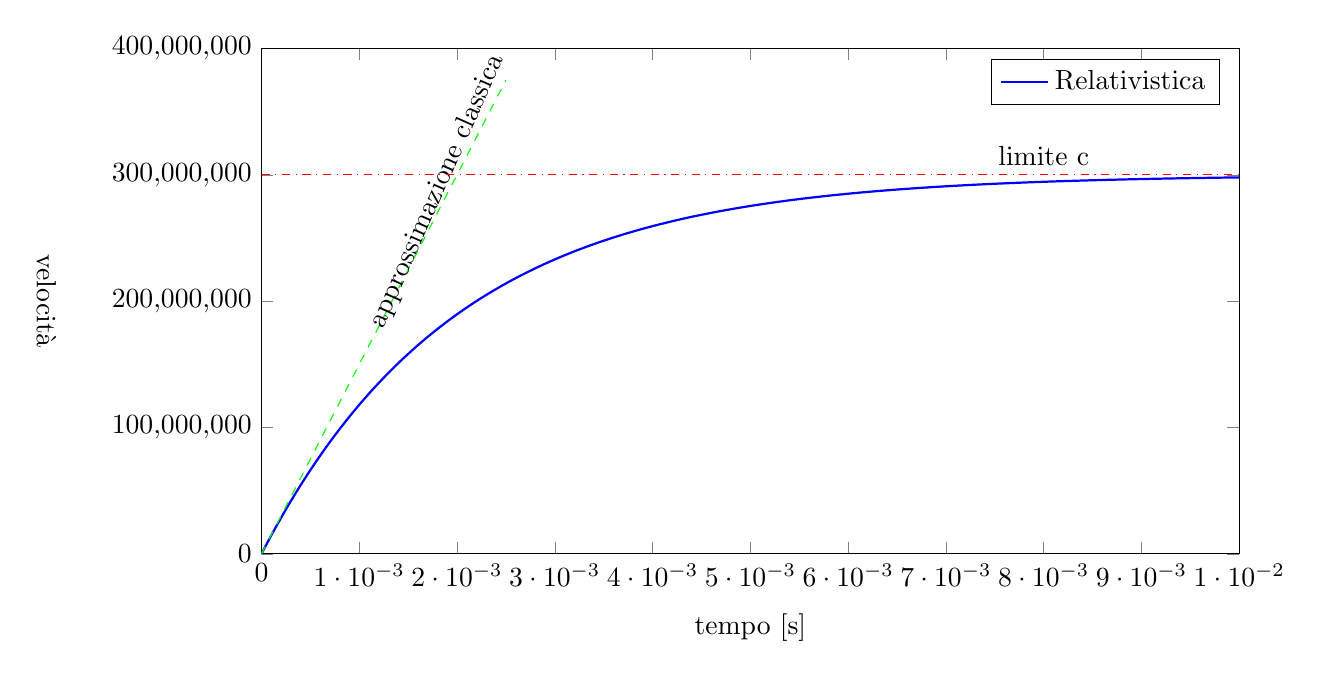
\begin{tikzpicture}
\begin{axis}[
    width=14cm,
    height=8cm,
    xlabel={tempo [s]},
    ylabel={velocità},
    xmin=0, xmax=0.01,
    ymin=0, ymax=4e8,
    xtick={0,0.001,0.002,0.003,0.004,0.005,0.006,0.007,0.008,0.009,0.01},
    yticklabel style={/pgf/number format/fixed},
    scaled y ticks=false,
    scaled x ticks=false,
    y label style={at={(axis description cs:-0.2,.5)},rotate=180},
    x label style={at={(axis description cs:0.5,-0.1)}},
]

% Parametri
\def\c{3e8} % velocità della luce
\def\a{1.5e11} % accelerazione costante (esempio)

% Curva relativistica (approssimazione)
\addplot[blue, thick, domain=0:0.01, samples=200] 
    {\c*(1 - exp(-\a*x/\c))}; % modello esponenziale per saturazione
\addlegendentry{Relativistica}

% Curva classica
\addplot[green, dashed, domain=0:0.0025, samples=100] 
    {\a*x};
\node[above, rotate=66] at (axis cs:0.002,2.8e8) {approssimazione classica};

% Linea limite c
\addplot[red, dash dot, domain=0:0.01] {\c};
\node[above] at (axis cs:0.008,3e8) {limite c};

\end{axis}
\end{tikzpicture}

\label{fig:2_velocitàTempo}
\caption{Andamento della velocità in funzione del tempo per particella accelerata}
\end{figure}

Nel limite classico, il concetto di massa inerziale coincide con quello di massa a riposo relativistico.